%%%%%%%%%%%%%%%%%%%%%%%%%%%%%%%%%%%%%%%%%%%%%%%%%%%%%%%%%%%%%%%%%%%%%%%%%%%%%%%%
%2345678901234567890123456789012345678901234567890123456789012345678901234567890
%        1         2         3         4         5         6         7         8

%\documentclass[journal,transmag]{IEEEtran}% Comment this line out if you need a4paper

\documentclass[10pt, conference]{ieeeconf}      % Use this line for a4 paper


\IEEEoverridecommandlockouts                              % This command is only needed if 
                                                          % you want to use the \thanks command

%\overrideIEEEmargins                                      % Needed to meet printer requirements.

% See the \addtolength command later in the file to balance the column lengths
% on the last page of the document

% The following packages can be found on http:\\www.ctan.org
%\usepackage{graphics} % for pdf, bitmapped graphics files
%\usepackage{epsfig} % for postscript graphics files
%\usepackage{mathptmx} % assumes new font selection scheme installed
%\usepackage{times} % assumes new font selection scheme installed
%\usepackage{amsmath} % assumes amsmath package installed
%\usepackage{amssymb}  % assumes amsmath package installed

\newtheorem{theorem}{Theorem}[section]
\newtheorem{lemma}[theorem]{Lemma}
\newtheorem{proposition}[theorem]{Proposition}
\newtheorem{corollary}[theorem]{Corollary}
\usepackage[ruled,vlined]{algorithm2e}
\usepackage{url}
\newenvironment{definition}[1][Definition]{\begin{trivlist}
\item[\hskip \labelsep {\bfseries #1}]}{\end{trivlist}}

\newcommand{\qed}{\nobreak \ifvmode \relax \else
      \ifdim\lastskip<1.5em \hskip-\lastskip
      \hskip1.5em plus0em minus0.5em \fi \nobreak
      \vrule height0.75em width0.5em depth0.25em\fi}

\def\lc{\left\lfloor}   
\def\rc{\right\rfloor}

\usepackage{amsmath,amssymb}

\usepackage{tabularx}
\usepackage{tikz,hyperref,graphicx,units}
\usepackage{subfigure}
\usepackage{benktools}
\usepackage{bbm}
\renewcommand{\baselinestretch}{.5}

\usepackage{caption}
\usepackage{epstopdf}
\renewcommand{\captionfont}{\footnotesize}
\usepackage{sidecap,wrapfig}
\usepackage[ruled,vlined]{algorithm2e}
\DeclareMathOperator*{\argmin}{arg\,min}
\DeclareMathOperator*{\argmax}{arg\,max}
\newcommand{\abs}[1]{\lvert#1\rvert} 
\newcommand{\norm}[1]{\lVert#1\rVert}
%\newcommand{\suchthat}{\mid}
\newcommand{\suchthat}{\ \big|\ }
\newcommand{\ba}{\mathbf{a}}
\newcommand{\bb}{\mathbf{b}}
\newcommand{\bc}{\mathbf{c}}
\newcommand{\bd}{\mathbf{d}}
\newcommand{\bg}{\mathbf{g}}
\newcommand{\bj}{\mathbf{j}}
\newcommand{\bn}{\mathbf{n}}
\newcommand{\bp}{\mathbf{p}}
\newcommand{\bw}{\mathbf{w}}
\newcommand{\bt}{\mathbf{t}}
\newcommand{\bu}{\mathbf{u}}
\newcommand{\by}{\mathbf{y}}
\newcommand{\bx}{\mathbf{x}}
\newcommand{\bz}{\mathbf{z}}
\newcommand{\bbf}{\mathbf{f}}
\newcommand{\bzero}{\mathbf{0}}
\newcommand{\bG}{\mathbf{G}}
\newcommand{\bA}{\mathbf{A}}
\newcommand{\bW}{\mathbf{W}}
\newcommand{\bX}{\mathbf{X}}
\newcommand{\mX}{\mathcal{X}}
\newcommand{\mD}{\mathcal{D}}
\newcommand{\mG}{\mathcal{G}}
\newcommand{\mN}{\mathcal{N}}
\newcommand{\mW}{\mathcal{W}}
\newcommand{\mF}{\mathcal{F}}
\newcommand{\bZ}{\mathbf{Z}}
\newcommand{\mR}{\mathcal{R}}

\newcommand{\bfc}{W}
\newcommand{\Qinf}{Q_{\infty}}
\newcommand{\st}[1]{_\text{#1}}
\newcommand{\rres}{r\st{res}}
\newcommand{\pos}[1]{(#1)^+}
\newcommand{\depth}{\operatorname{depth}}
\newcommand{\dist}{\operatorname{dist}}
\newcommand{\convhull}{\operatorname{ConvexHull}}
\newcommand{\minksum}{\operatorname{MinkowskiSum}}

\newcommand{\specialcell}[2][c]{ \begin{tabular}[#1]{@{}c@{}}#2\end{tabular}}
\newcommand{\acro}{SHIV}
\newcommand\independent{\protect\mathpalette{\protect\independenT}{\perp}}
\def\independenT#1#2{\mathrel{\rlap{$#1#2$}\mkern2mu{#1#2}}}

\newcolumntype{L}[1]{>{\RaggedRight\hspace{0pt}}p{#1}}
\newcolumntype{R}[1]{>{\RaggedLeft\hspace{0pt}}p{#1}}


\newboolean{include-notes}
\setboolean{include-notes}{true}
\newcommand{\adnote}[1]{\ifthenelse{ \boolean{include-notes}}%
 {\textcolor{blue}{\textbf{AD: #1}}}{}}
 
 \newcommand{\fpnote}[1]{\ifthenelse{ \boolean{include-notes}}%
 {\textcolor{blue}{\textbf{FP: #1}}}{}}
 
  \newcommand{\mlnote}[1]{\ifthenelse{ \boolean{include-notes}}%
 {\textcolor{purple}{\textbf{ML: #1}}}{}}

\renewcommand{\baselinestretch}{.95}
\usepackage{times}
\usepackage{microtype}
%\title{Iterative Imitation Learning with Reduced Human Supervision [v11]}
%\title{SHIV:  Reducing Human Supervision for Robot Active Learning [v11]}

\title{Robotic Grasping in Clutter: Using a Hierarchy of Supervisors with  (Deep) Learning from Demonstrations}



\author{Michael Laskey$^1$, Jonathan Lee$^1$, Caleb Chuck$^1$, David Gealy$^1$, Wesley Hsieh$^1$, Florian T. Pokorny,\\
 Anca D. Dragan$^1$, and Ken Goldberg$^{1,2}$% <-this % stops a space
\thanks{$^1$ Department of Electrical Engineering and Computer Sciences; {\small \{mdlaskey,iamwesleyhsieh,ftpokorny,anca\}@berkeley.edu, \small staszass@rose-hulman.edu} }%
\thanks{$^2$ Department of Industrial Engineering and Operations Research; {\small goldberg@berkeley.edu}}%
\thanks{$^{1-2}$ University of California, Berkeley;  Berkeley, CA 94720, USA}%
}
\begin{document}



\maketitle
\thispagestyle{empty}
\pagestyle{empty}


%%%%%%%%%%%%%%%%%%%%%%%%%%%%%%%%%%%%%%%%%%%%%%%%%%%%%%%%%%%%%%%%%%%%%%%%%%%%%%%%

\begin{abstract}
Recent progress in learning from demonstrations increasingly indicates that robots can acquire manipulation skills from
large collections of training data. Online learning from demonstration algorithms such as DAgger can in particular learn
policies for problems where the system dynamics and the cost function are unknown. Traditionally, these systems have
been trained by skilled human supervisors providing feedback on the current learned policy. As the number of
demonstrations increases, this approach can however incur a substantial time and labor cost. We propose that a hierarchy of supervisors that vary is expertise but also in cost can help alleviate this issue. We combine planning on a relaxed problem with crowdsourcing and with robotics experts, and hypothesize that leveraging this combination can lead to similar performance while substantially decreasing cost. We focus on the grasping in clutter problem, and use an architecture for learning from demonstration based on DAgger and deep learning to learn policies directly from image input. Our results ....[fill in]

 \end{abstract}


%%%%%%%%%%%%%%%%%%%%%%%%%%%%%%%%%%%%%%%%%%%%%%%%%%%%%%%%%%%%%%%%%%%%%%%%%%%%%%%%

\section{Introduction} 
As illustrated by the recent Amazon Picking Challenge at ICRA 2015, the grasping in clutter problem, where a robot needs
to grasp an object that might be occluded by other objects in the environment poses an interesting challenge to robotic
systems. Two fundamental approaches to grasping in clutter include the analytic model driven approach \cite{1,2,3},
where the interaction dynamics between the robot and obstacles are formulated analytically. However, modeling all the 
physical properties of interaction poses a highly challenging problem due to uncertainty in modeling parameters such as
inertial properties and friction. 

Another approach to the grasping in
clutter problem in a data-driven manner, where the interaction behavior is learned directly from interactions with the environment and a supervisor, which can be an expert human or an analytical method \cite{argall2009survey}. Learning from demonstration (LfD) algorithms have been used
successfully in recent years for a large number of robotic tasks, including helicopter
maneuvering~\cite{abbeel2007application}, car parking~\cite{abbeel2008apprenticeship},  and robot
surgery~\cite{van2010superhuman}. Furthermore, deep learning, which we use to learn policies directly from raw video
data, has emerged as a highly versatile technique used for this purpose ~\cite{pinto2015supersizing}.

\begin{figure}
\includegraphics[width=0.5\textwidth]{f_figs/teaser.eps}
\caption{
Three roll-outs on a Zymark 3-DOF Robot of a fully trained grasping in clutter policy (one per column, bottom to top) which was trained using a
hierarchy of three supervisors consisting of an analytical motion planning, crowd-sourcing and human expert. 
Red shapes indicate clutter objects and the robot is trained to reach the yellow circle. The trained manipulation policy is represented as a deep neural network that recieves as input an image of the scene and outputs a change in state position. The resulting policy learns to sweep away clutter objects and reach the goal object. }
\vspace*{-20pt}
\label{fig:teaser}
\end{figure}

%LfD algorithms can be categorized as either \emph{offline}, where the robot only observes a set of finalized
%demonstrations, or \emph{online}, where the robot rolls out a current policy and then receives feedback from the supervisor.
%In offline LfD, the robot learns the policy based on a batch of examples, and then executes it to achieve the task.  During execution, 
%control error can accumulate, leading the robot away from the region of the state space where it was provided with
%training data, leading to unpredictable behavior. For example, an autonomous car trained on examples of a cars driving
%near the center of a lane might, due to deviations encounter new states far away from previously trained examples that
%can result in failures~\cite{pomerleau1989alvinn}. For a class of supervised learning methods, Ross and Bagnell showed
%that the number of errors made by the robot, can scale quadratically with the time horizon of the task, in particular~\cite{ross2010efficient}.

Our approach is based on online Learning from Demonstrations (LfD) where a robot iteratively learns a policy and is
provided by feedback on the current policy roll out by a supervisor~\cite{grollman2007dogged,ross2010efficient,ross2010reduction}. 
We build on, DAgger, an online LfD algorithm which at each iteration, computes a policy based on prior demonstrations,
and then rolls out that policy. A supervisor then provides control signals as feedback on the current policy
and new state/control examples are aggregated with the prior examples for the next iteration. DAgger and related algorithms have been applied in a wide range of applications, from quadrotor flight to natural language to Atari games~\cite{NIPS2014_5421,duvallet2013imitation,ross2013learning}. 
Ross et al. showed that DAgger, under a no-regret assumption, can be guaranteed to deviate from the supervisor's policy with an error
at most linear in the time horizon for the task~\cite{ross2010reduction}.

One drawback is that DAgger imposes a substantial burden on the supervisor, who must label all states that the robot
visits during training.  Traditionally there has only been one supervisor and it is deemed an expert
~\cite{ross2010efficient,ross2010reduction,ross2013learning,duvallet2013imitation}. In this work, we propose to instead
utilize a hierarchy of supervisors that exhibit increasing cost and competence at a given task to incrementally
bootstrap the learning process. 

In particular, while model-based planners might not yet capture the full physical interaction among all objects, it can be wasteful to not leverage them and learn with an expert supervisor from scratch. Thus, at the lowest lever of the hierarchy, we use a motion planner on an relaxed version of the problem. In our grasping application, we use a planner that ignores the obstacles but can leverage knowledge of the kinematics and the goal.
The next supervisor in the hierarchy are crowdsource workers on Amazan Mechnical Turk. Then finally the robot is trained with a Phd student in robotics, who is an expert human supervisor. Examples of the resulting learned grasping in clutter policy can be seen in Fig. \ref{fig:teaser}. 

%Learning can be bootstrapped with a sequence of increasingly skilled supervisors. In our grasping in clutter example, the robot spends a large portion of the time learning how to go towards the goal object. Analytical techniques such as forward kinematics, template matching and motion planning are readily available to provide examples in these parts of the state space. 

%We propose bootstrapping a policy from a hierarchy of supervisors ranked by cost: analytical models, crowd-sourced workers and an expert supervisor to learn the robot grasping in clutter task. We demonstrate this approach by training a deep neural network for the visuo-motor based task of  grasping in clutter on a Zymark Robot. Our robot consists of an 2DOF arm and a gripper that lie in a planar workspace. The objects dataset consists of 20  extruded polygons taken from 2D projections of objects in the Dex-Net \cite{mahler2016dexnet} database.  Results show that by leveraging a hierarchy of less skilled experts, the total amount of cost incurred is reduced by X$\%$ and the task is $61\%$ successful on our test set of 20 object configurations of shapes not trained on \mlnote{need to think of a better teaser statement}


\section{Related Work}
Below, we summarize related work in Robotic Grasiping in Clutter, the Online LfD setting and then the field of
Curriculum learning, which is related to the concept of hierarchical supervisors.\adnote{make sure to talk about guided policy search too, which is a way to combine deep nets with either human or planner supervision}

\noindent \textbf{Robotic Grasping in Clutter}
Robotic grasping is a well-established research topic in robotics that has been studied for several
decades~\cite{bicchi2000robotic}. A significant amount of prior work focuses on planning grasps given a known object.
However, in unstructured environments clutter poses a significant challenge for reaching the planned grasp
~\cite{katz2008can}. Prior work has addressed integrated perception and grasping in clutter where the objective is to
grasp objects in an unorganized pile ~\cite{pinto2015supersizing,nieuwenhuisen2013mobile}, but these methods do not
specifically aim to grasp a single target object in clutter. Leeper et al. ~\cite{} use a human operator for assistance
to guide the robot through clutter with the objective of grasping a target object. However, the robot required the human
to be present at all times and did not attempt to learn to operate autonomously. We are interested in a data-driven
approach that only queries a supervisor at training time and which can operate autonomously thereafter.

Prior work has studied the problem of manipulating objects
by performing pushing operations~\cite{}. Berenson et
al. ~\cite{} in particular use a sampling-based planner that considers clearance
from obstacles in the environment to plan a grasp
approach trajectory in cluttered environments. Cosgun et al.
[3] and King et al. \cite{kingnonprehensile} consider the problem of planning
a series of push operations that move an object to a
desired target location. Kiteav et al. planned a trajectory in a physics simulator using LQG based controllers
\cite{kitaevphysics}. However, all of these works assume a known model of of the object behavior is provided. We are
interested in learning manipulation polices in a data-driven manner instead, leveraging a hierarchy of supervisors for
training.  
\mlnote{We should discuss how to distinguish our work (Properties of our approach are we assume raw image data, real time and unknown dynamics)}. 

\noindent \textbf{Online Lfd with an Expert Supervisor}
Successful robotic examples of Online Learning From Demonstration with an expert supervisor include applications to flying a quad-copter through a forest, navigating a wheel chair across a room and teaching a robot to follow verbal instructions and surgical needle insertion \cite{ross2013learning, kim2013maximum, duvallet2013imitation, laskey}. 

However, to date, these approaches have used only one expert supervisor to provide training data for all parts of the
state space. We propose to instead utilize hierarchy of supervisor of different skill level and cost to reduce the
overall learning cost. 

\noindent\textbf{Reducing Supervisor Burden in Online LfD} One approach that has been studied to reduce the number of
supervisor supervision is to apply active learning to only ask for supervision when the robot is uncertain about the
correct control to apply. Traditional active learning techniques like query-by-committee and uncertainty sampling have
in particular be utilized for this purpose \cite{chernova2009interactive,judah2011active,grollman2007dogged}

However, Kim et al. demonstrated that due to the non-stationarity of the distribution of states encountered during
learning, the traditional active learning techniques may be suitable since the underlying state distribution changes.
Thus the use of novelty detection was proposed~\cite{kim2013maximum}. Laskey et al. introduced SHIV, using an active
learning approach tailored to high dimensional and non-stationarity state distributions and a modified version of the
One Class SVM classifier. This enabled the authors to reduce the density estimation problem to a 
simpler regularized binary classification~\cite{laskey}. However the grasping in clutter problem exhibits a high amount
of stochasticity requiring a large training data set which poses a significant computational challenge to these methods.
In the present paper, we hence consider using Deep Learning, as an underlying scalable learning algorithm in combination
with DAgger.

\noindent\textbf{Curriculum Learning}
Our approach is closely related to ideas from curriculum learning, where a neural network is trained via 
incrementally, first on easier examples and then gradually on data of increasing difficulty~\cite{bengio2009curriculum}.

Sanger et al. used curriculum learning in robotics to gradually train a neural network policy to learn the inverse
dynamics of a robot manipulator. They then considered a collection scheme where easily learned trajectories where shown
to the robot first and then gradually increased the difficulty~\cite{sanger1994neural}.

Our approach is different from curriculum learning, which assumes all training data presented to the neural network is valid.  We  instead train on a completely different set of examples throughout the supervisor hierarchy.  In these different set of examples, some could be very low-quality examples and will enforce a behavior that needs to be retrain with a more-skilled supervisor. 

\section{Problem Statement}
Given a collection of increasingly able and costly supervisors $S_1, \ldots, S_M$, the goal of this work is to learn a
policy that closely matches that of the most able supervisor $S_M$ while minimizing the overall cost of training a
policy. We formalize this approach as follows.

\noindent\textbf{Assumptions and Modeling Choices } 
We assume a known state space and set of controls. We also assume access to a robot or simulator, such that we  can sample from the state sequences induced by a sequence of controls.Lastly, we assume access to a set of supervisors who can, given a state, provide a control signal label. We additionally assume the supervisors can be noisy and imperfect, noting that a lower cost supervisor also has lower quality.

 We model the system dynamics as Markovian, stochastic, and stationary. Stationary dynamics occur when, given a state and a control, the probability of the next state does not change over time. Note this is different from the non-stationary distribution over the states the robot encounters during learning. We model the initial state as sampled from a distribution over the state space. 


\noindent\textbf{Policies and State Densities.}
Following conventions from control theory, we denote by $\mathcal{X}$ the set of observable states for a robot task, consisting, for example, of 
high-dimensional vectors corresponding to images from a camera, or robot joint angles and object poses in the environment.
We denote by $\mathcal{U}$ the set of allowable control inputs for the robot. $\mathcal{U}$ may be discrete or
continuous in nature. We model dynamics as Markovian: the probability of state $\mathbf{x_{t+1}}\in
\mathcal{X}$ depends only oni the previous state $\mathbf{x}_t\in\mathcal{X}$ and control input $\mathbf{u}_t\in
\mathcal{U}$: 
$$p(\bx_{t+1}|\bu_{t},\bx_{t}, \ldots, \bu_{0}, \bx_{0})=p(\bx_{t+1}|\bu_{t}, \bx_t)$$
We assume an unknown probability density over initial states $p(\bx_0)$.

A demonstration (or trajectory) $\hat{\tau}$ is a series of $T+1$ pairs of states visited and corresponding
control inputs at these states, $\hat{\tau} = (\mathbf{x}_0,\mathbf{u}_0, ...., \mathbf{x}_T,\mathbf{u}_T)$, where $\bx_t\in \mathcal{X}$
and $\bu_t\in \mathcal{U}$ for $t\in \{0, \ldots, T\}$ and some $T\in \mathbb{N}$.  
For a given trajectory $\hat{\tau}$ as above, we denote by ${\tau}$ the corresponding trajectory in state space,
${\tau} = (\bx_0,....,\bx_T)$.

A policy is a function $\pi: \mathcal{X} \to \mathcal{U}$ from states to control inputs. 
We consider a space of policies $\pi_{\theta}:\mathcal{X}\to \mathcal{U}$ parameterized by some $\theta\in \mathbb{R}^d$. Any such policy $\pi_{\theta}$ in an environment with probabilistic initial state density and Markovian dynamics
induces a density on trajectories. Let $p(\bx_t|\theta)$ denote the value of the density of states visited at time $t$ if the robot follows the policy $\pi_{\theta}$ from time $0$ to time $t-1$.  Following~\cite{ross2010reduction}, we can compute
the average density on states for any timepoint by $p(\bx|\theta) = \frac{1}{T} \sum^T_{t=1} p(\bx_t|\theta)$.

While we do not assume knowledge of the distributions corresponding to: $p(\bx_{t+1}|\bx_t,\bu_t)$, $p(\bx_0)$, $p(\bx_t|
\theta)$ or $p(\bx|\theta)$, we assume that we have a stochastic robot or a simulator such that for any state
$\bx_t$ and control $\bu_t$, we can sample the $\bx_{t+1}$ from the density $p(\bx_{t+1}|\pi_{\theta}(\bx_t),\bx_t)$. 
Therefore, 'rolling out' trajectories under a policy
$\pi_{\theta}$ in our experiments, we utilize the robot to sample the resulting stochastic trajectories rather than
estimating $p(\bx|\theta)$ itself.

{\color{blue} FP: might make this and the above specific to grasping in clutter?}
\noindent\textbf{Objective.} The objective of policy learning is to find a policy that maximizes some known cumulative
reward function $\sum^T_{t=1} r(\bx_t,\bu_t)$ of a trajectory $\hat{\tau}$. The reward $r:\mathcal{X}\times
\mathcal{U}\to \mathbb{R}$ is typically user defined and task specific \cite{1,2,3}. 
For example, in the task of inserting a peg into a hole, a function quantifying a notion of distance between the peg's
current and desired final state can be used~\cite{levine2015end}.  

Since grasp success is typically considered as a binary reward which is observed only at a delayed final state \cite{kitaevphysics}, 
grasping in clutter poses a challenging problem for traditional reinforcement learning methods. We hence instead build
upon DAgger which queries a supervisor for appropiate actions, to provide the robot a set of N stochastic demonstrations trajectories $\lbrace \hat{\tau}^1,...\hat{\tau}^N \rbrace$. This induces a training data set $\mathcal{D}$ of state-control input pairs. 
We define a `surrogate' loss function as in~\cite{ross2010reduction}, $l:\mathcal{U}\times \mathcal{U}\to \mathbb{R}$, which provides a distance
measure between any pair of control values. We consider $l(\bu_0,\bu_1) = ||\bu_0-\bu_1||^2_2$.

Given a candidate policy $\pi_{\theta}$, we DAgger uses the surrogate loss function to approximately measure how `close' the robot's policy's
returned control input $\pi_{\theta}(\bx)\in \mathcal{U}$ at a given state $\bx\in \mathcal{X}$ is to the supervisor's policy's control output
$\tilde{\pi}(\bx)\in \mathcal{U}$. The goal is of DAgger is to produce a policy that minimizes the expected surrogate loss:


 \vspace{-2ex}
\begin{align}\label{eq:LFD_obj}
\underset{\theta}{\min} \: E_{p(\bx|\theta)} [l(\pi_\theta(\bx),\tilde{\pi}(\bx))]
\end{align}

Instead of a single supervisor $S$, which classically is considered to be a skilled human teacher, we instead consider a
hierarchy $S_1, \ldots, S_M$ of supervisors which we may be algorithms or humans and which follow policies $\pi_1, \ldots, \pi_M$ with
associated expected cumulative rewards $R_i$ satisfying $R_1\le R_2 \le \ldots \le
R_M$. Furthermore, we assume that the cost associated to providing a state
label for supervisor $S_i$ is $C_i$ with $C_1\le C_2 \le \ldots C_M$, so that the ordering of supervisors is consistent
with respect to both cost and skill level. We consider the problem of minimizing the expected surrogate loss of a
trained policy with respect to the most skilled supervisor $S_M$ in the hierarchy while minimizing the overall training
cost.

 In particular, this paper provides an empirical study of greedy combinations of three types of supervisors $S_1,
S_2, S_3$ for grasping in clutter which are applied in order to train a policy parameterized by a deep neural network.
Here, $S_1$ is an analytical motion planning algorithm with a cost $C_1=0.01$, $S_2$ a supervisor
consisting a crowd-sourced Amazon Mechanical Turk laborers with $C_2=0.1$, and $S_3$ a human expert supervisor with
$C_3=1$.

\section{Approach and Background}
 \subsection{Details on DAgger: Dataset Aggregation}
Since the cumulative expected reward of a policy is difficult to optimize directly,
DAgger~\cite{ross2010reduction} instead solves the minimization in Eq. \ref{eq:LFD_obj} by iterating two steps: 1)
computing the policy parameter $\theta$ using the training data $\mathcal{D}$ thus far, and 2) execute the policy induced by the current $\theta$, and ask for labels for the encountered states. 
 
\subsubsection{Step 1}
The first step of any iteration $k$ is to compute a $\theta_k$ that minimizes surrogate loss on the current dataset $\mathcal{D}_k=\{(x_i,u_i)|i\in\{1,\ldots,M\}\}$ of demonstrated state-control pairs (initially just the set $\mathcal{D}$ of initial trajectory demonstrations):

 \vspace{-1ex}
\begin{align}\label{eq:super_objj}
\theta_{k} = \underset{\theta}{\argmin} \: \sum_{i=1}^{M} l(\pi_{\theta}(\bx_i),\bu_i).
\end{align}

This sub-problem is a supervised learning problem, solvable by estimators like a support vector machine or a neural net. Performance can vary though with the selection of a the estimator~ Selecting the correct function class depends on the task being consider and knowledge of the problem, see for a guide~\cite{scholkopf2002learning}. 
 

 \subsubsection{Step 2}
The second step  DAgger rolls out their policies, $\pi_{\theta_{k}}$, to sample states that are likely under $p(\bx|\theta_{k})$.  For every state visited, DAgger requests the supervisor to provide the appropriate control/label. Formally, for a given sampled trajectory  $\hat{\tau} = (\bx_0,\bu_0,...,\bx_T,\bu_T )$, the supervisor provides labels $\tilde{\bu}_t$, where $\tilde{\bu}_t \sim \tilde{\pi}(\bx_t) + \epsilon$, where $\epsilon$ is a small zero mean noise term, for $t\in \{0, \ldots, T\}$.
The states and labeled controls are then aggregated into the next data set of demonstrations $\mathcal{D}_{k+1}$:
$$D_{k+1}=\mathcal{D}_k \cup \{(\bx_t,\tilde{\bu_t})\|t\in\{0,\ldots,T\}\} $$

%\fpnote{terms such as aggregated etc would be much clearer if we just refer to a particular line in the algorithm}

Steps 1 and 2 are repeated for $K$ iterations or until 
the robot has achieved sufficient performance on the task\footnote{In the original DAgger the policy rolled out
was stochastically mixed with the supervisor, thus with probability $\beta$ it would either take the supervisor's action
or the robots. The use of this stochastically mix policy was for theoretical analysis. In practice, it is recommended
to set $\beta = 0$ to avoid biasing the sampling~\cite{NIPS2014_5421,ross2010reduction}}.


\subsection{DAgger with Supervisor Hierarchy}
Formulating a framework for supervisor strategy selection poses a challenging problem since no formal model
for the effect of supervisor selection on the surrogate loss minimization is available a priori and since the
neural network policy parameters $\theta$ are additionally changing at each step of DAgger's iterative training process.

While one could consider to learn a policy using model-free reinforcement learning algorithms
~\cite{sutton1998reinforcement}, where a selection strategy will query different supervisors and learn over time the
best supervisor to select given the current policy, this approach requires substantial numbers of 
queries for supervision of the costliest supervisor at each iteration. In light of this, we propose a greedy allocation
strategy.

We train a policy with the cheapest supervisor $S_1$ for a fixed number of $K_1$ iterations with DAgger and then advance
linearly through the hierarchy $S_1, \ldots, S_M$, where the final Neural Network Parameters $\theta_i$ trained using
$S_i$ are transferred iteratively to supervisor $S_{i+1}$ before further training the policy with DAgger.
Each supervisor is trained for $K_i, i\in \{1, \ldots, M\}$ iterations in turn. 

While for large numbers of iterations, convergence tests can be applied to determine a point of diminishing return at
which a switch to the next supervisor in the hierarchy can be initiated, this approach can be challenging when only a
limited numbers of roll-outs can be afforded. In practice, we either advanced when the surrogate loss between
supervisors was sufficiently low or when the performance on the grasping in clutter task was not improving empirically. 
For crowdsourcing in particular, we chose the second option since, due to the large variance between demonstrations
we were not able to determine a fixed threshold for the surrogate loss. We hope to significantly scale the number of
training steps in future work to investigate various switching criterea in full detail.

\begin{figure}[t]
\centering

\includegraphics[width=\columnwidth, height=4cm]{f_figs/labeling.pdf}

\caption{\footnotesize  The interface AMT workers see for providing feedback to the robot for the grasping in clutter task. The pink overlay indicates the desire change in the robot position with respect to the current robot state. Then AMT workers can use their intuition for how objects respond to force to provide examples of how the robot should behave. Each window shows a correction in a degree of freedom a) is the rotation of the robots base b) is extending the robot's arm.}
\vspace*{-10pt}
\label{fig:overlays}
\end{figure}


\section{Robot Grasping in Clutter}
We now describe the grasping in clutter problem, the supervisor hierarchy that we used to solve it and our deep learning policy architecture. 

\subsection{Grasping in Clutter}\label{sec:task}
Consider a robot in an Amazon warehouse. The robot has an intended goal object for it to grasp on a shelf, however other objects could obstruct the path towards the goal object. These obstructions of movable objects prevent leveraging common motion planning techniques, because they do not posses a dynamics model of how the objects behave under different contact forces. ~\cite{kitaevphysics,kingnonprehensile}.

Thus, the robot must reason about how its interactions with the environment will affect the intended outcome. This can be hard for two reasons 1) it becomes hard to find a low dimensional state representation for the task because the environment dynamics are affected by the global shape of each object 2) the dynamics of the environment  involve modeling how K objects interact with each other under an arbitrary force \cite{kitaevphysics}.

In order to achieve real time grasping in clutter, which is important for a robot in a shipping warehouse, we leverage  visuo-motor deep learning to learn a control policy for the task over a large number of different configurations working with a hierarchy of supervisors. Deep learning has the potential to take high dimensional image data of the scene and learn task specific features relevant for grasping in clutter. Additionally a trained neural network policy is can be computational inexpensive to evaluate and can result in real time performance \cite{levine2015end}.

\subsection{Supervisor Hierarchy}\label{sec:hier}
In this section, we list each supervisor in the order they appear in our hierarchy. The first supervisor is deemed the least expensive. 

\noindent \textbf{Motion Planning that Ignores Obstacles Supervisor} Our first supervisor, $S_1$, is a a motion planner that that computes the trajectory the robot should move in to reach the goal object, or yellow circle, by ignoring obstacles.  Thus we refer to $S_1$ as Motion Planning that Ignores Obstacle (MPIO) supervisor. Our method employs template matching to identify the goal object in the image and the using the forward dynamics of the robot to computes the relative change in direction the robot should apply as an control. The template matching is implemented in OpenCV and uses the normalized cross-correlation filter~\cite{opencv_library}.

In this stage, the MPIO supervisors only tries to teach the robot to move towards the goal. Note that the MPIO supervisor's examples does not have any knowledge about how the cluttered objects will respond to the forces applied via the robot arm, which results in sub-optimal polices. However, the MPIO supervisor is both computationally and monetarily inexpensive to run which allows us to provide a large number of examples. Thus, the cost of the MPIO supervisor is $C_1 = 0.01$. 


\noindent \textbf{CrowdSourced Supervisor} The second supervisor, $S_2$, relies on a crowd source service, called Amazon Mechanical Turk (AMT). The AMT platform makes readily available thousands of human workers that can perform  provide examples for  \$0.12 per robot trial. Thus potentially providing a higher quality supervisor who has an intuition for how the cluttered objects interact with the world, but at a  higher cost, $C_2 = 0.1$.

In order to get examples from a CrowdSourced Supervisor, we designed an interface shown in Fig. \ref{fig:overlays}. The interface draws a transparent overlay that shows how the robot would respond provided the current control Thus, allowing for the AMT worker to see the magnitude and effect their example would have on the robot.

We additionally designed a tutorial for the CrowdSourced Supervisor. First, we introduce them to a robot named Izzy and briefly explain that Izzy is trying to reach a yellow circle but has a tendency to "misbehave" and needs their help. Then we have them perform designated motions with a virtual Izzy, which helps them understand how the robot's dynamics behave. We additionally provide a video of an expert providing corrections on three robot trajectories. We lastly instruct the CrowdSourced Supervisor to only label when they are sure in their decision, in order to prevent contradictory examples associated with them second guessing themselves.  

While completing a tutorial before providing examples can be beneficial, we still are not sure whether the CrowdSourced Supervisor can provide quality examples that can be used in learning. To help ensure quality, we give all CrowdSourced Supervisor  the same robot trial first and measure their examples against the examples form a  Human Expert Supervisor. If the average Squared-Euclidean distance between examples is above a threshold of the Human Expert's examples or the number of examples they provided is above a threshold of the number the Human Expert provided, the Crowdsource Supervisor is not asked to provide additional examples.



\noindent \textbf{Human Expert Supervisor} The final supervisor, $S_3$ is the Human Expert supervisor, who is capable of achieving high cumulative reward but is a limited resource. An Human Expert Supervisor in this case is a Phd student in machine learning and robotics, which costs $C_3=1.0$. The Human Expert Supervisor uses the same interface , shown in Fig. \ref{fig:overlays}, to provide examples to the robot.  

An expert supervisor can be used in a variety of scenarios.They first would have a better intuition of the physical limitations of the robot and environment, such as joint limits or how certain objects might behave under force. Furthermore, they would also understand how the examples given could lead to better training of the robot's policy $\pi_\theta$. For example, understanding the feature space the policy lies in can lead the Human Expert to not providing contradictory examples. 



\subsection{Neural Network Policy Architecture}
\mlnote{adding more details with figure tomorrow}
Our policy is represented as deep neural network, which was trained using TensorFlow~\cite{tensorflow2015-whitepaper}. Our network architecture consists of 1 convolutional layer with 5 channels and filters with size 11x11, a fully connected layer with an output of 128 dimensions and a final layer that maps to a four dimensional control signal. We used ReLus to separate the different layers and a final tanh on the output to scale the output between -1 and 1. 

The control examples was scaled between 1 and -1 for each dimension independently. To be robust to lighting and reduce the dimensionality of the problem, we applied a binary mask to each channel of the 250x250 RGB image, the mask would set to 1 values above 125 and 0 other wise.  We then validated that all information (i.e. location of the gripper, cluttered shapes and goal object) where still visible in the masked image. 

To determine our architecture we preformed a grid search over different architectures  trained after 400 iterations with a batch size of 200. The set of architectures consist of different network architectures as well as different momentum terms, and weight initialization schemes. We trained all networks on a dataset of 6K images labeled with the Analytical Supervisor on a Nvidia Tesla K40 GPU, which is able to train each network in an average of 10 minutes.  


\section{Experiments} \label{sec:Exp}
\begin{figure}[t]
\centering

\includegraphics{f_figs/robot.eps}

\caption{\footnotesize  Shown above is a Zymark robot. The robot consists of an 3DOF arm that lies in a planar workspace and the ability to rotate the turn table. The inscribed circle in the work space prevents the robot from learning the trivial policy of just pushing the objects off the table.}

\label{fig:robot}
\end{figure}

\begin{figure}[t]
\centering
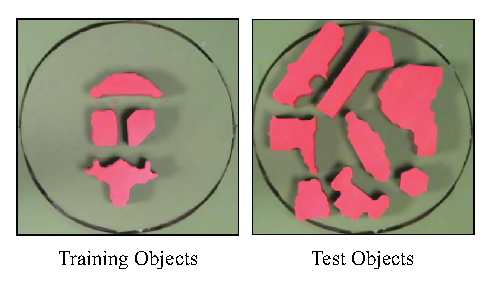
\includegraphics{f_figs/shapes_set.eps}

\caption{\footnotesize  The set of objects that the robot was trained on. The Training objects on the right are the four objects used in training. The test objects on the left represent represent objects that were found in our test configurations. The test objects vary in size and shape from the training objects, which can test how well the robot learns to manipulate unknown objects. Every test configuration contained at least one object from this set to guarantee it wasn't trained on.  }

\label{fig:shape_set}
\end{figure}


\begin{figure}[t]
\centering
\includegraphics{f_figs/succes_measure.eps}

\caption{\footnotesize  The different measure of success used in our scoring metric for how well the robot performed.  Not successful corresponds to when the gripper is never in contact with yellow circle. Near successful corresponds to when the robot ends with the gripper touching the yellow circle. Successful is defined as when the yellow circle is inside the gripper. }
\vspace*{-20pt}
\label{fig:suc_meas}
\end{figure}


In this section, we first describe the grasping in clutter experimental setup. Then we test how the supervisor hierarchy performs versus not leveraging a hierarchy. We then test how high of Quality the CrowdSource supervisor is. Then, we experiment with different ways to advance in the hierarchy. Finally, we look at using all three supervisors and to train a robot for the grasping in clutter task. 

\subsection{Experimental Setup}
For experimenting in the grasping in clutter domain, we are interested in training a Zymark robot to perform a grasping in clutter task on image data taken from a Logitech C270 camera. Examples of images from the camera can be seen in Fig. \ref{fig:teaser}.

The objects in clutter are made Medium Density Fiberboard and each one is on average 4" in diameter. The objects deemed cluttered are painted Red and the goal object is painted yellow. There is an inscribed circle around the work space to keep the robot from pushing the objects outside of the work space. The inscribed circle can make the task more challenging because the robot cannot simply "sweep" the cluttered objects off the table. 

The robot, shown in Fig. \ref{fig:robot}, has a 3 dimensional internal state of base rotation, arm extension and gripper. The robot is commanded via state position requests, which are tracked by a tuned PID controller. We used relative state contorl because 1) it is easier to enforce stay out zones (such as where a human operator could be) in the robot configuration space and 2) registering state control to a labeling interface in Fig. \ref{fig:overlays} is more straightforward than motor commands.   The policy $\pi_\theta$ outputs delta positions that are bounded by $15^\circ$ for the gripper and turntable, $1$ cm for the arm extension and $0.5$ cm for the gripper at each time step. There is $T=100$ time steps in a trajectory. 

To test the performance of a policy, we created a test set composed of 20 different configurations each containing objects that were not trained on.  The test set configurations varied in number of objects on the table, size of objects and relative pose of each object. The objects that were trained on and those that were only tested on can be seen in Fig. \ref{fig:shape_set}.  We measure success as defined by three situations not successful, near successful, successful. Examples of the robot in these situations can be seen in Fig. \ref{fig:suc_meas}. 

The not successful situation corresponds to the case when the robot's gripper is not touching the goal object at the end of a rollout. Examples of when this happens is when the robot fails to push the objects away or does not head in the direction of the yellow circle. The near successful situation is defined as the robot touches the goal object with its gripper, but it is not enclosed in the gripper. Examples of when this happens is when the robot gets a small obstacle object trapped in the gripper first, or when the root slightly misses the yellow circle on its approach. Successful is defined as getting the goal object inside the gripper at the end of a trajectory. We report total success as a score out of 2: 0 for not successful, 1 for near successful, 2 for successful. 

In all experiments we used a batch size of 20 trials per iterations or 2000 images, thus 100 trials corresponds to 5 iterations. 

\subsection{Hierarchical Supervisors}

\begin{figure*}[t]
\centering
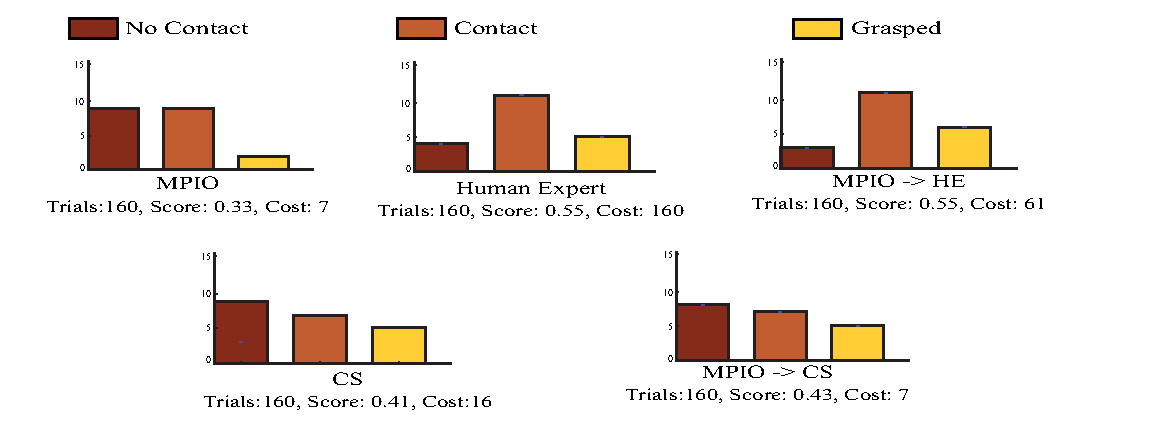
\includegraphics{f_figs/results.eps}

\caption{ \footnotesize The performance and cost of each policy trained with a supervisor is reported. The bar graphs shows the breakdown in terms of situations the policy encountered on the test set. The top row corresponds to policies only trained with one supervisor: MPIO, Crowdsourced or Human Expert. The bottom corresponds to policies trained with a hierarchy of supervisors: MPIO and Crowdsource, MPIO and Human Expert, MPIO, Crowdsourced and Human Expert. The final bottom right plot demonstrates the full hierarchy, which achieves the best performance (0.8).   }
\vspace*{-20pt}
\label{fig:perf_results}
\end{figure*}
\adnote{reorder: mpio, he, mpio->he (main experiment); then cs, mpio-cs, all; cs is missing score, hopefully it does not much better than mpio-cs; don't highlight bottom right option because technically its not suppoed to be better than expert; just use hypotheses to show your points.; also separate mpio-cs-he from rest becuase it is using double the data! not fair comparison! spread the legend horizontally at the top; }


We first test  that using a hierarchy of supervisors can reduce total cost needed to train a policy, but still maintain similar performance .  We compare having only a MPIO Supervisor for a fixed amount of data to having only an Human Expert, and to having the hierarchy of both . The non-hierarchical policies trained with the human expert supervisor only for 160 demonstrations or only the MPIO supervisor for 160 demonstrations.  The policy trained with a hierarchical supervisor first receives  100 demonstrations from the MPIO supervisor and  60 demonstrations from the expert supervisor. 

Our results, shown in Fig. \ref{fig:perf_results}, are the policy trained with just the MPIO supervisor achieves a score of $0.325\%$, the policy trained with just an expert achieves $0.54\%$ and the policy trained with a hierarchy of supervisor achieves $0.55\%$.  Thus, the hierarchical supervisor and expert supervisor achieve approximately the same performance. However,training with a hierarchical supervisor yields a $40\%$ reduction in cost incurred compared to the policy trained with only an expert supervisor. 


Thus demonstrating that by using a hierarchy of supervisors, we can reduce the cost of training a policy and achieve similar performance to the Human Expert Supervisor.


\begin{figure}[t]


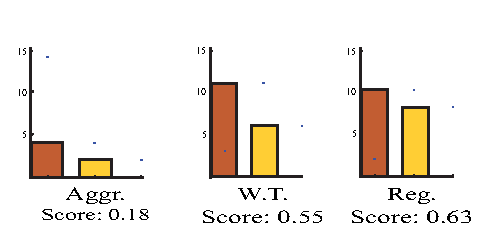
\includegraphics{f_figs/cost_result.eps}

\caption{\footnotesize The performance of each policy trained with a different data management strategy is reported. The bar graphs shows the breakdown in terms of situations the policy encountered on the test set. Each policy was trained with the MPIO to Human Expert hierarchical supervisor. From left to right is the following data management strategies: Dataset Aggregation, Weight Transfer and Regularization. Regularization achieves the highest performing score of (0.18) }
\label{fig:cost_result}
\end{figure}

\subsection{Quality of Crowdsourced Supervisor}
We next evaluate the potential of a  crowdsourced supervisor for a being part of the hierarchy. Thus, we perform an experiment using the AMT platform described in Sec. \ref{sec:hier}. We  first test how well a crowdosurce supervisor performs as part of a hierarchy of supervisors. We trained a policy with 100  demonstrations  from the MPIO supervisor , then had 60 demonstrations provided by AMT workers. We also compare how well the crowdsource supervisors performs just as well as a single supervisor,  by having them provide all 160 demonstrations.

Our results, shown in Fig. \ref{fig:perf_results}, are the policy trained with just the crowdsourced supervisor achieves a score of $?\%$. The policy trained with the hierarchical crowdsourced and MPIO supervisor receives $0.43\%$ on our test set compared to $0.55\%$ with the motion planning and expert supervisors hierarchy. The total cost received with the only crowdsource supervisor was 15, while the hierarchical supervisor was 7. 

In total, we tested on 44 AMT workers. We asked them to provide examples for a single rollout and then if they passed quality check asked them if they wanted to exit or continue for an additional \$$0.12$ per demonstration. We found only 21 AMT workers were able to pass the quality check and continue providing demonstrations. On average a worker would provide 4 demonstrations before exiting the AMT HIT. 

\subsection{Advancing in the Hierarchy}
We further test how to advance between supervisors in the hierarchy.We examine three different strategies for dataset management when changing supervisors 1) aggregating the dataset of the data collected with both supervisors 2) transferring only the weights of the nerural network policy or $\theta$ vector between the supervisors and removing the first's supervisors dataset completely 3) transferring only the weights of the neural network policy but adding the values output by $\pi_\theta(\bx)$  instead of $\tilde{\pi}_m(\bx)$at parts of the states visited that the current supervisor is close to agreement with as measured by the following $||\tilde{\pi}_m(\bx) - \pi_\theta(\bx)||^2_2 < 0.01$. Thus, acting as a regularization on the optimization since stochastic gradient on a section of the min-batch update would be zero for examples where the next supervisor agrees with the previous. 


We compare each strategy on a hierarchy of a MPIO supervisor trained with 100 iterations and then advancing to a human expert supervisor trained with 60 iterations.  Our results reported in Fig.\ref{fig:cost_result} , show that aggregation strategy achieves $0.18\%$, the weight transfer strategy achieves $0.55\%$ and the regularized stochastic gradient update strategy achieves $0.63\%$. Thus, suggesting that techniques to help the policy remain close to the previously trained supervisor are useful for effectively switching between supervisors.   



An issue arises though when performing this iterations because now the current dataset $\mathcal{D}_{K_m}$ has examples from a different supervisor that receives a smaller expected cumulative reward. This could cause a learning algorithm to try and fit to contradictory examples  and be worse than either supervisor trained with \cite{scholkopf2002learning}.

We are thus interested in not storing the dataset collected from the previous supervisor and only remembering the current $\theta_{m,K}$ weight parameters. Thus, we propose only performing DAgger for each individual supervisor in the hierarchy and using the resulting weight vector to bootstrap the learning of the next supervisor. We found empirically in Sec. \ref{sec:Exp} that it also beneficial to add to the new dataset the states and controls applied by the current policy $\pi_{\theta_{m,k}}$ that the current supervisor agreed with by some euclidean distance $\tilde{\epsilon}$.Thus, acting as a regularization on the optimization since stochastic gradient on a section of the min-batch update would be zero for examples where the next supervisor agrees with the previous. 



\subsection{Scaling the Hierarchy}
The final experiment we ran is to run our algorithm on a hierarchy with 3 supervisors: MPIO, crowdsourced and human expert. We ran each policy until we observed the pay out in terms of reward achieved was not increasing. This results in MPIO for 100 demonstrations, crowdsourced for 120 demonstrations and human expert for 100 demonstrations. Thus resulting in 320 trials on the robot and 320,000 annotated images of what control the robot should apply. 

The results of our trained policy, as shown in Fig. \ref{fig:perf_results}, demonstrate that by leveraging a hierarchy we are able to achieve a score of $80\%$ with a cost of only 113. We note that policy trained with the human expert supervisor, which incurred a cost of $160$, was only able to achieve a score of $0.66\%$. 

While our policy was able to do substantially better, it did score a near successful  $40\%$. These failure modes where do to the robot not being able to accurately manipulate smaller objects, where slight perturbations could result them being pushed into the gripper, and accurately controlling the goal object to land in the circle (i.e. sometimes pushing against the side of the circle instead). We attribute this problem to a limit in the detail of precision our supervisors can currently give, future work will look at more precise analytical methods and fine tuning the policies via self-learning. 


\begin{figure}[t]
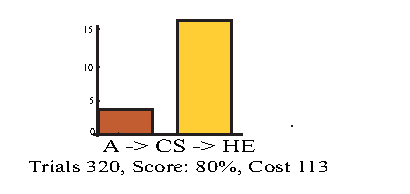
\includegraphics{f_figs/big_data.eps}

\caption{ \footnotesize The performance and cost of each policy trained with a supervisor is reported. The bar graphs shows the breakdown in terms of situations the policy encountered on the test set. The top row corresponds to policies only trained with one supervisor: MPIO, Crowdsourced or Human Expert. The bottom corresponds to policies trained with a hierarchy of supervisors: MPIO and Crowdsource, MPIO and Human Expert, MPIO, Crowdsourced and Human Expert. The final bottom right plot demonstrates the full hierarchy, which achieves the best performance (0.8).   }
\vspace*{-20pt}
\label{fig:big_data}
\end{figure}

\section{Discussions and Future Work}
For highly stochastic domains like grasping in clutter, using a hierarchy of supervisors to bootstrap performance at a lower cost seems to be a very sensible thing to do. Our results suggest that we can scale up the amount of data needed to learn the task at a much lower cost than only querying the most-skilled supervisor. However, much work still needs to be done in determining how to appropriately select the next supervisor to receive examples from. While our current strategy worked well empirically, it remains to be seen if this would apply to other domains. 

Future work will also look at how to increase the success rate on the grasping in clutter domains. The current failure modes are associated with a lack of fine motor precision. Our current supervisors do not  have the ability to give finer motor control corrections, however using more sophisticated analytical methods might enable better performance. Furthermore, applying self-learning  to our current policy could be a way to "fine-tune" the current behavior and learn the precision. 




 \section{Acknowledgments} 
This research was performed in UC Berkeley's Automation Sciences Lab under the UC Berkeley Center for Information Technology in the Interest of Society (CITRIS) "People and Robots" Initiative. This work is supported in part by the U.S. National Science Foundation under Award IIS-1227536, NSF-Graduate Research Fellowship, by the Knut and Alice Wallenberg Foundation and the National Defense Science and Engineering Graduate Fellowship Program. We thank Steve McKinely and Meng Guo for help in building the hardware setup.  

  
\bibliographystyle{IEEEtranS}
\bibliography{references}



\end{document}
%\subsection{Hierarchies} If the robot could learn the policy  perfectly, this state density would match the one encountered in user examples. But if the robot makes an error, that error changes the distribution of states that the robot will visit, which can lead to states that are far away from any examples and difficult to generalize to~\cite{pomerleau1989alvinn}. This motivates iterative algorithms like DAgger, which iterate between learning a policy and the supervisor providing examples. We  introduce the concept of their being a set of supervisors each with an associated cost and skill level. Denote $\tilde{\pi}_M$ the most skilled and costly supervisor in this set. This supervisor could for example be a person with a Phd in machine learning and robotics. We formally define how each supervisor in the set is related to each other in Sec. \ref{sec:hS}.  Every time a supervisor is queried a cost, $C_m$, is incurred this could be an hourly pay rate or computational time. While Eq. \ref{eq:LFD_obj} is the primary objective of our algorithm a secondary objective is to reduce the cumulative cost associated with training the robot. Thus, we are interested in solving the following objective

%where $J$ is the number of queries need to satisfy the constraint on expected surrogate loss, $C_{m,j}$ denotes the cost incurred by querying the supervisor at that iteration and $\epsilon$ is a user-defined threshold on how close robot policy is to match the highest quality supervisor. We present our algorithm, LEATHERMAN, which aims to solve Eq. \ref{eq:bugjet_LFD_obj}.
 

%\subsection{Hierarchy of Supervisors}\label{sec:hS} Instead of one  supervisor,we propose a hierarchy  of $M$ supervisors where for each supervisor $\tilde{\pi}_m$, there is an associated expected cumulative reward $R_m = \int \sum^T_{t=1} r(\mathbf{x}_t, \tilde{\pi}_m(x)) p(\tau |\tilde{\pi}_m)d\tau$, where $p(\tau |\tilde{\pi}_m)$ denotes the average distribution of states the supervisor encounters. We also denote some measure of cost $C_m$ that is ascribed to the supervisor, such as computational time or monetary expense. Generally the rank of supervisors in terms of cost is equivalent to the rank of supervisor in the terms of expected cumulative reward. Thus, the least costly supervisor will receive the lowest expected cumulative reward. 

%Additionally for two supervisors $\tilde{\pi}_m$ and $\tilde{\pi}_{m+1}$ to be in the hierarchy, they must only disagree in expectation on a subset of the work space to some precision $\tilde{\epsilon}$. Denote the set of states two supervisors disagree as $\mathcal{X}_{m,m+1} = \lbrace \mathbf{x} | ||\tilde{\pi}_m(\mathbf{x}) - \tilde{\pi}_{m+1}(\mathbf{x}) ||^2_2 > \tilde{\epsilon} \rbrace$ .We enforce the condition $\mathcal{X}_{m,m+1} \subset \mathcal{X}$ because if two supervisors never provided the same examples then all states would have to be relabeled by the next supervisor in the hierarchy. 

%We formally define an ordering on supervisors:

%\begin{definition} Two supervisors $\tilde{\pi}_m$ and $\tilde{\pi}_{m+1}$ are in a hierarchy if  $C_m < C_{m+1}$  and  $\mathcal{X}_{m,m+1} \subset \mathcal{X}$ \end{definition}

%Violation of this definition could result in no additional benefit from the LEATHERMAN algorithm or potentially worst a higher budget incurred than without using a hierarchy of supervisors.
